\section{Data Augmentation Can Improve Robustness}

\begin{frame}{Data Augmentation Can Improve Robustness}
    \begin{figure}
        \centering
        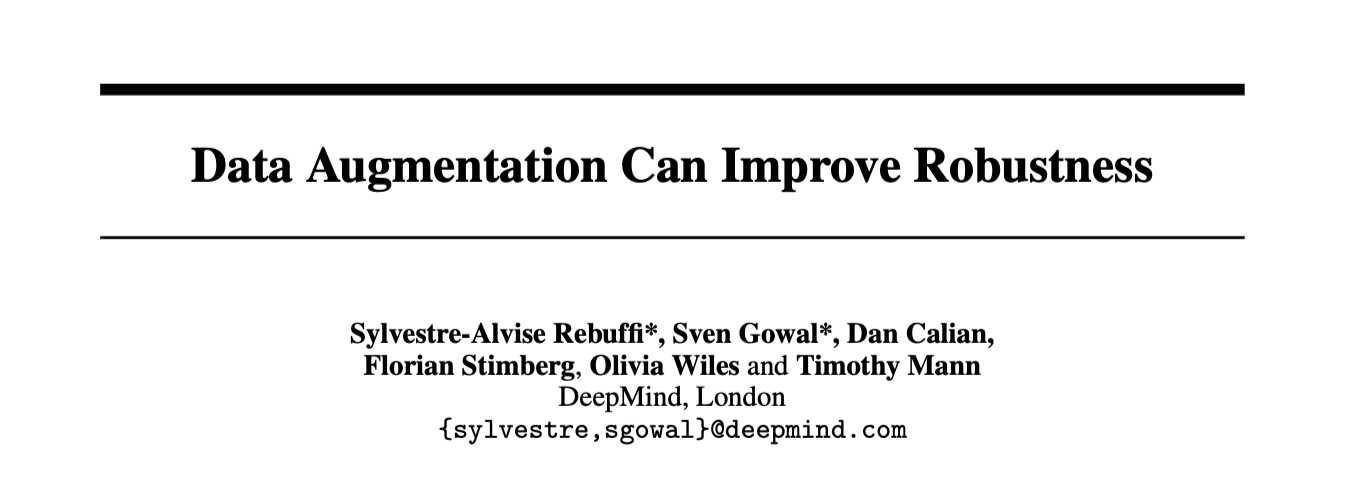
\includegraphics[width=\linewidth]{pic/Title.png}
        % \caption{Caption}
        \label{fig:title}
    \end{figure}
\end{frame}

\begin{frame}{Contributions}
    \begin{itemize}
        \item We demonstrate that, when combined with model weight averaging, data augmentation techniques such as \textit{Cutout}, \textit{CutMix} and \textit{MixUp} can improve robustness.
        \item To the contrary of \href{https://arxiv.org/pdf/2010.03593}{Gowal et al.}, Rice et al., Wu et al. we are able to use any of these three aforementioned techniques to obtain new \emph{state-of-the-art robust accuracies}. 
        \begin{figure}
            \begin{minipage}[c]{0.45\linewidth}
                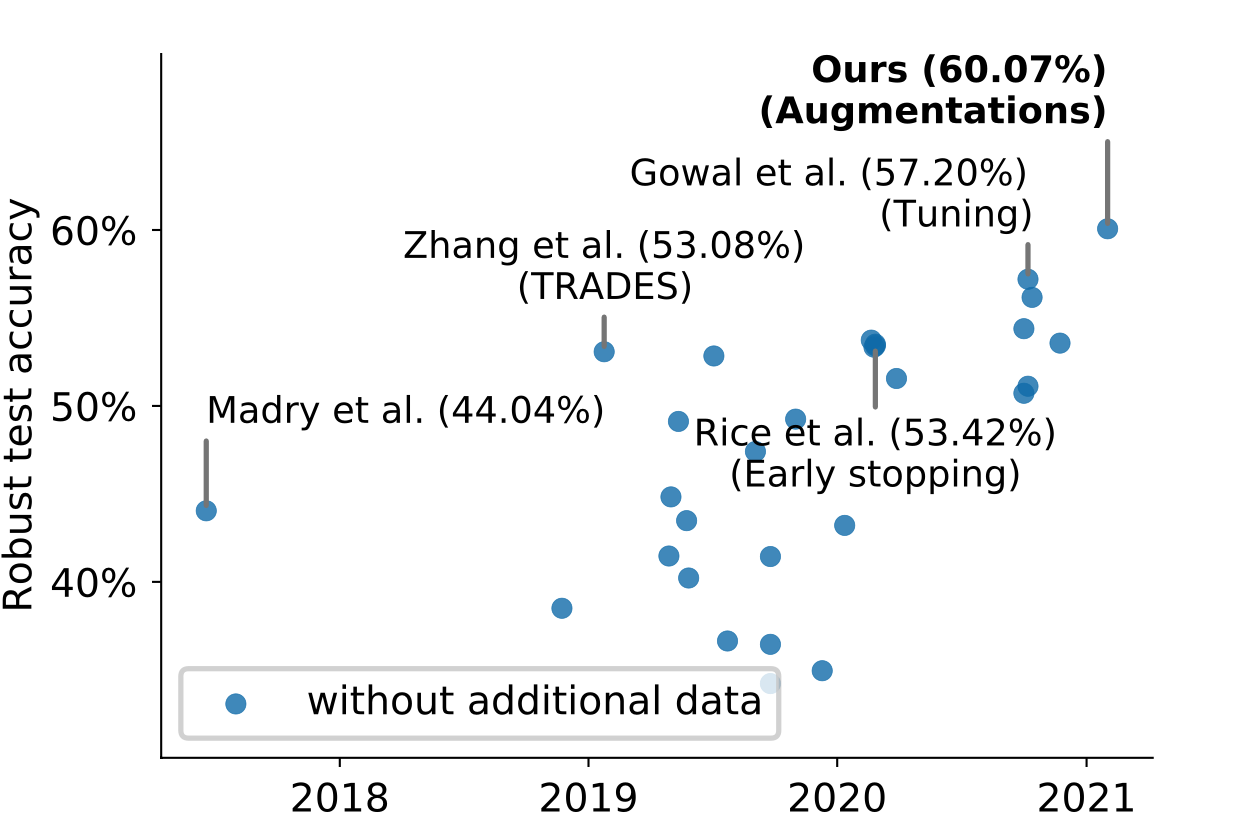
\includegraphics[width=\linewidth]{pic/sota.png}
            \end{minipage}
            \begin{minipage}[c]{0.45\textwidth}
                \caption{Robust accuracy of various models submitted to RobustBench against AUTOATTACK on CIFAR-10 with $\ell_\infty$ perturbations of size $8/255$ displayed in publication order. Our method builds on \href{https://arxiv.org/pdf/2010.03593}{Gowal et al.} and explores how augmented data can be used to improve robust accuracy by $+2.87\%$ without using any additional external data.} \label{fig:sota}
            \end{minipage}
        \end{figure}
        \item We show that our approach generalizes across architectures, datasets and threat models.
        \item We also investigate the trade-off between robust overfitting and underfitting to explain why \textit{MixUp} performs worse than spatial composition techniques.
        \item We provide empirical evidence that WA exploits data augmentation by ensembling model snapshots.
    \end{itemize}
\end{frame}

\begin{frame}{Hypothesis}
    \begin{itemize}
        \item As WA results in flatter, wider solutions compared to the steep decrease in robust accuracy observed for SGD, it is natural to ask ourselves whether WA remains useful in cases that do not exhibit robust overfitting.
        \item We notice that the robust performance in this setting is not only preserved but even boosted when using WA. 
        \item Hence, we formulate the hypothesis that: 
            \begin{quote}
                \emph{model weight averaging helps robustness to a greater extent when robust accuracy between model iterations can be maintained.}
            \end{quote}
        \item This hypothesis is also motivated by the observation that WA acts as a temporal ensemble – akin to Fast Geometric Ensembling by \href{https://arxiv.org/pdf/1802.10026}{Garipov et al.} who show that efficient ensembling can be obtained by aggregating multiple checkpoint parameters at different training times.
    \end{itemize}
\end{frame}

\begin{frame}{Limiting Robust Overfitting Without External Data}
    \begin{itemize}
        \item Rice et al. show that combining data augmentation methods such as \textit{Cutout} or \textit{MixUp} with early stopping does not improve robustness upon early stopping alone. 
        \item While, these methods do not improve upon the “best” robust accuracy, they reduce the extent of robust overfitting, thus resulting in a slower decrease in robust accuracy compared to classical adversarial training (which uses random crops and weight decay). 
        \begin{figure}
            \begin{minipage}[c]{0.6\linewidth}
                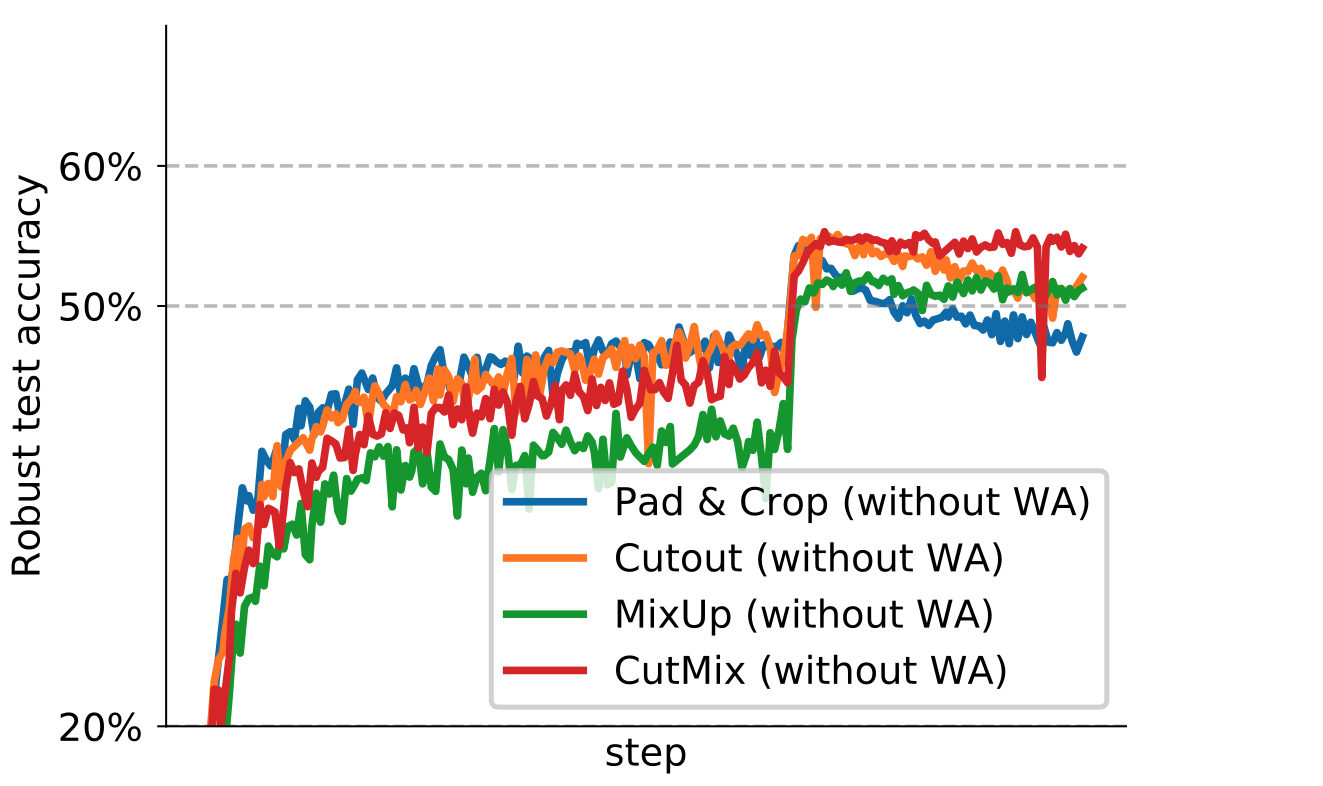
\includegraphics[height=.4\textheight]{pic/data_aug.png}
            \end{minipage}
            \begin{minipage}[c]{0.35\linewidth}
                \caption{Accuracy against $\epsilon_\infty = 8/255$ on CIFAR-10 without using model WA for different data augmentation schemes. The model is a WRN-28-10 and the panel shows the evolution of the robust accuracy as training progresses (against $PGD^{40}$). The jump in robust accuracy two-thirds through training is due to a drop in learning rate.}\label{fig:data_aug}
            \end{minipage}
        \end{figure}
    \end{itemize}
\end{frame}

\begin{frame}{Testing the Hypothesis}
    \begin{itemize}
        \item Since \textit{MixUp} preserves robust accuracy while \textit{Pad \& Crop} does not, this comparison can be used to evaluate the hypothesis that WA is more beneficial when the performance between model iterations is maintained.
        \begin{figure}
            \centering
            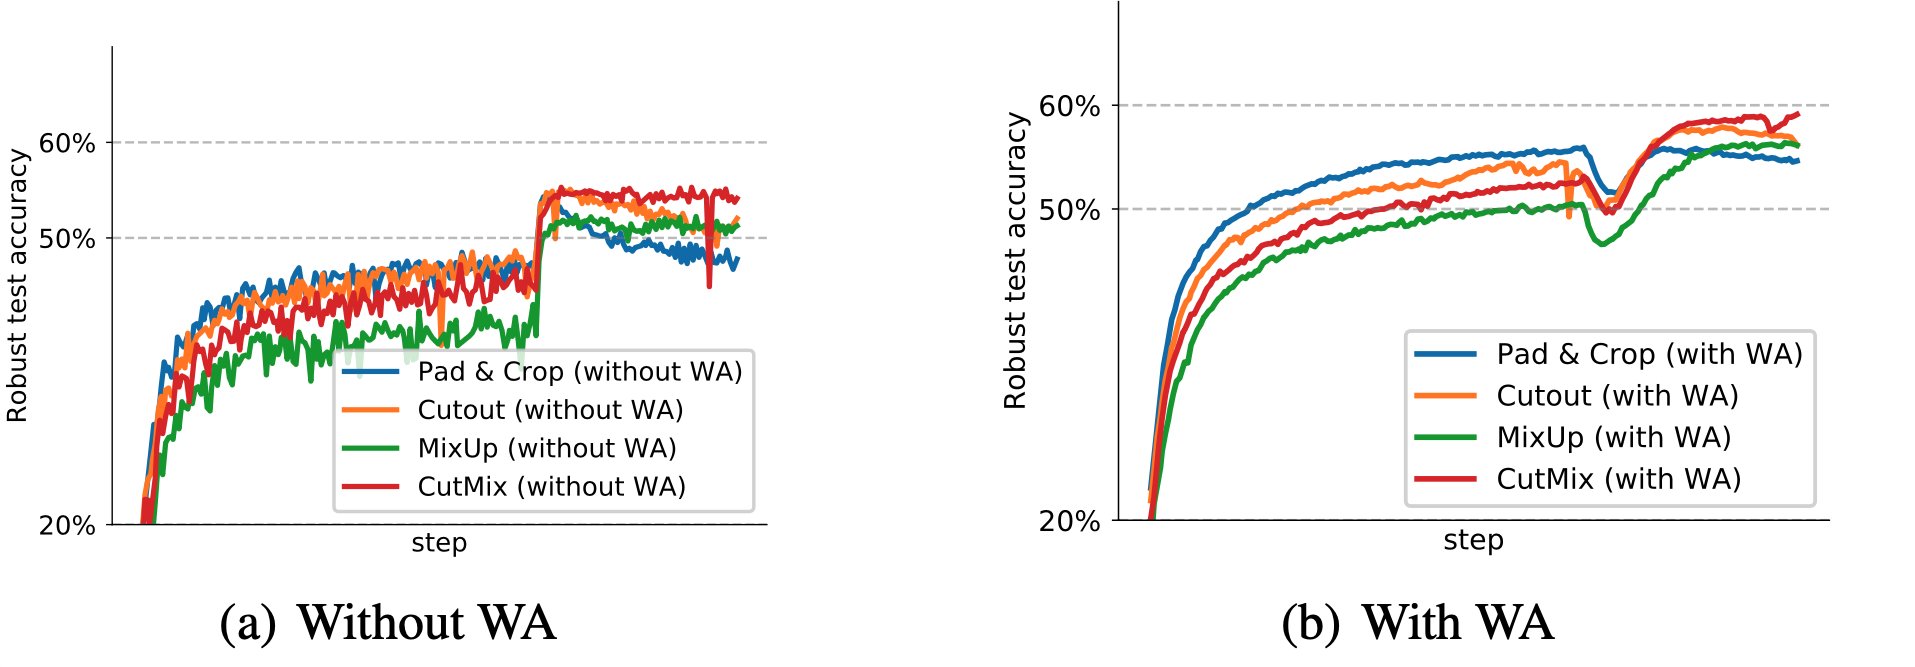
\includegraphics[height=.4\textheight]{pic/data_aug_wa.png}
            \caption{Accuracy against $\epsilon_\infty = 8/255$ on CIFAR-10 without using model weight averaging (WA) for different data augmentation schemes. The model is a WRN-28-10 and both panels show the evolution of the robust accuracy as training progresses (against $PGD^{40}$). The jump in robust accuracy two-thirds through training is due to a drop in learning rate. The accuracy drop just after the change of learning rate stems from averaging very different weights.}
            \label{fig:data_aug_wa}
        \end{figure}
    \end{itemize}
\end{frame}

\begin{frame}{Experimental Setup}
    \begin{itemize}
        \item \textbf{Architecture.} We use WRNs as our backbone network. Most of the experiments are conducted on a WRN-28-10 model which has a depth of 28, a width multiplier of 10 and contains 36M parameters. To evaluate the effect of data augmentations on wider and deeper networks, we also run several experiments using WRN-70-16, which contains 267M parameters.
        \item \textbf{Outer minimization.} We use TRADES optimized using SGD with Nesterov momentum and a global weight decay of $5 \times 10^{-4}$.
        \item \textbf{Inner minimization.} Adversarial examples are obtained by maximizing the Kullback-Leibler divergence between the predictions made on clean inputs and those made on adversarial inputs. 
        \item \textbf{Evaluation.} We train two (and only two) models for each hyperparameter setting, perform early stopping for each model on a separate validation set using $PGD^{40}$. Finally, we report the robust test accuracy against a mixture of AUTOATTACK and MULTITARGETED, which is denoted by AA+MT.
    \end{itemize}
\end{frame}